\vspace{-1.5em}
\begin{figure}[H]
    \centering
    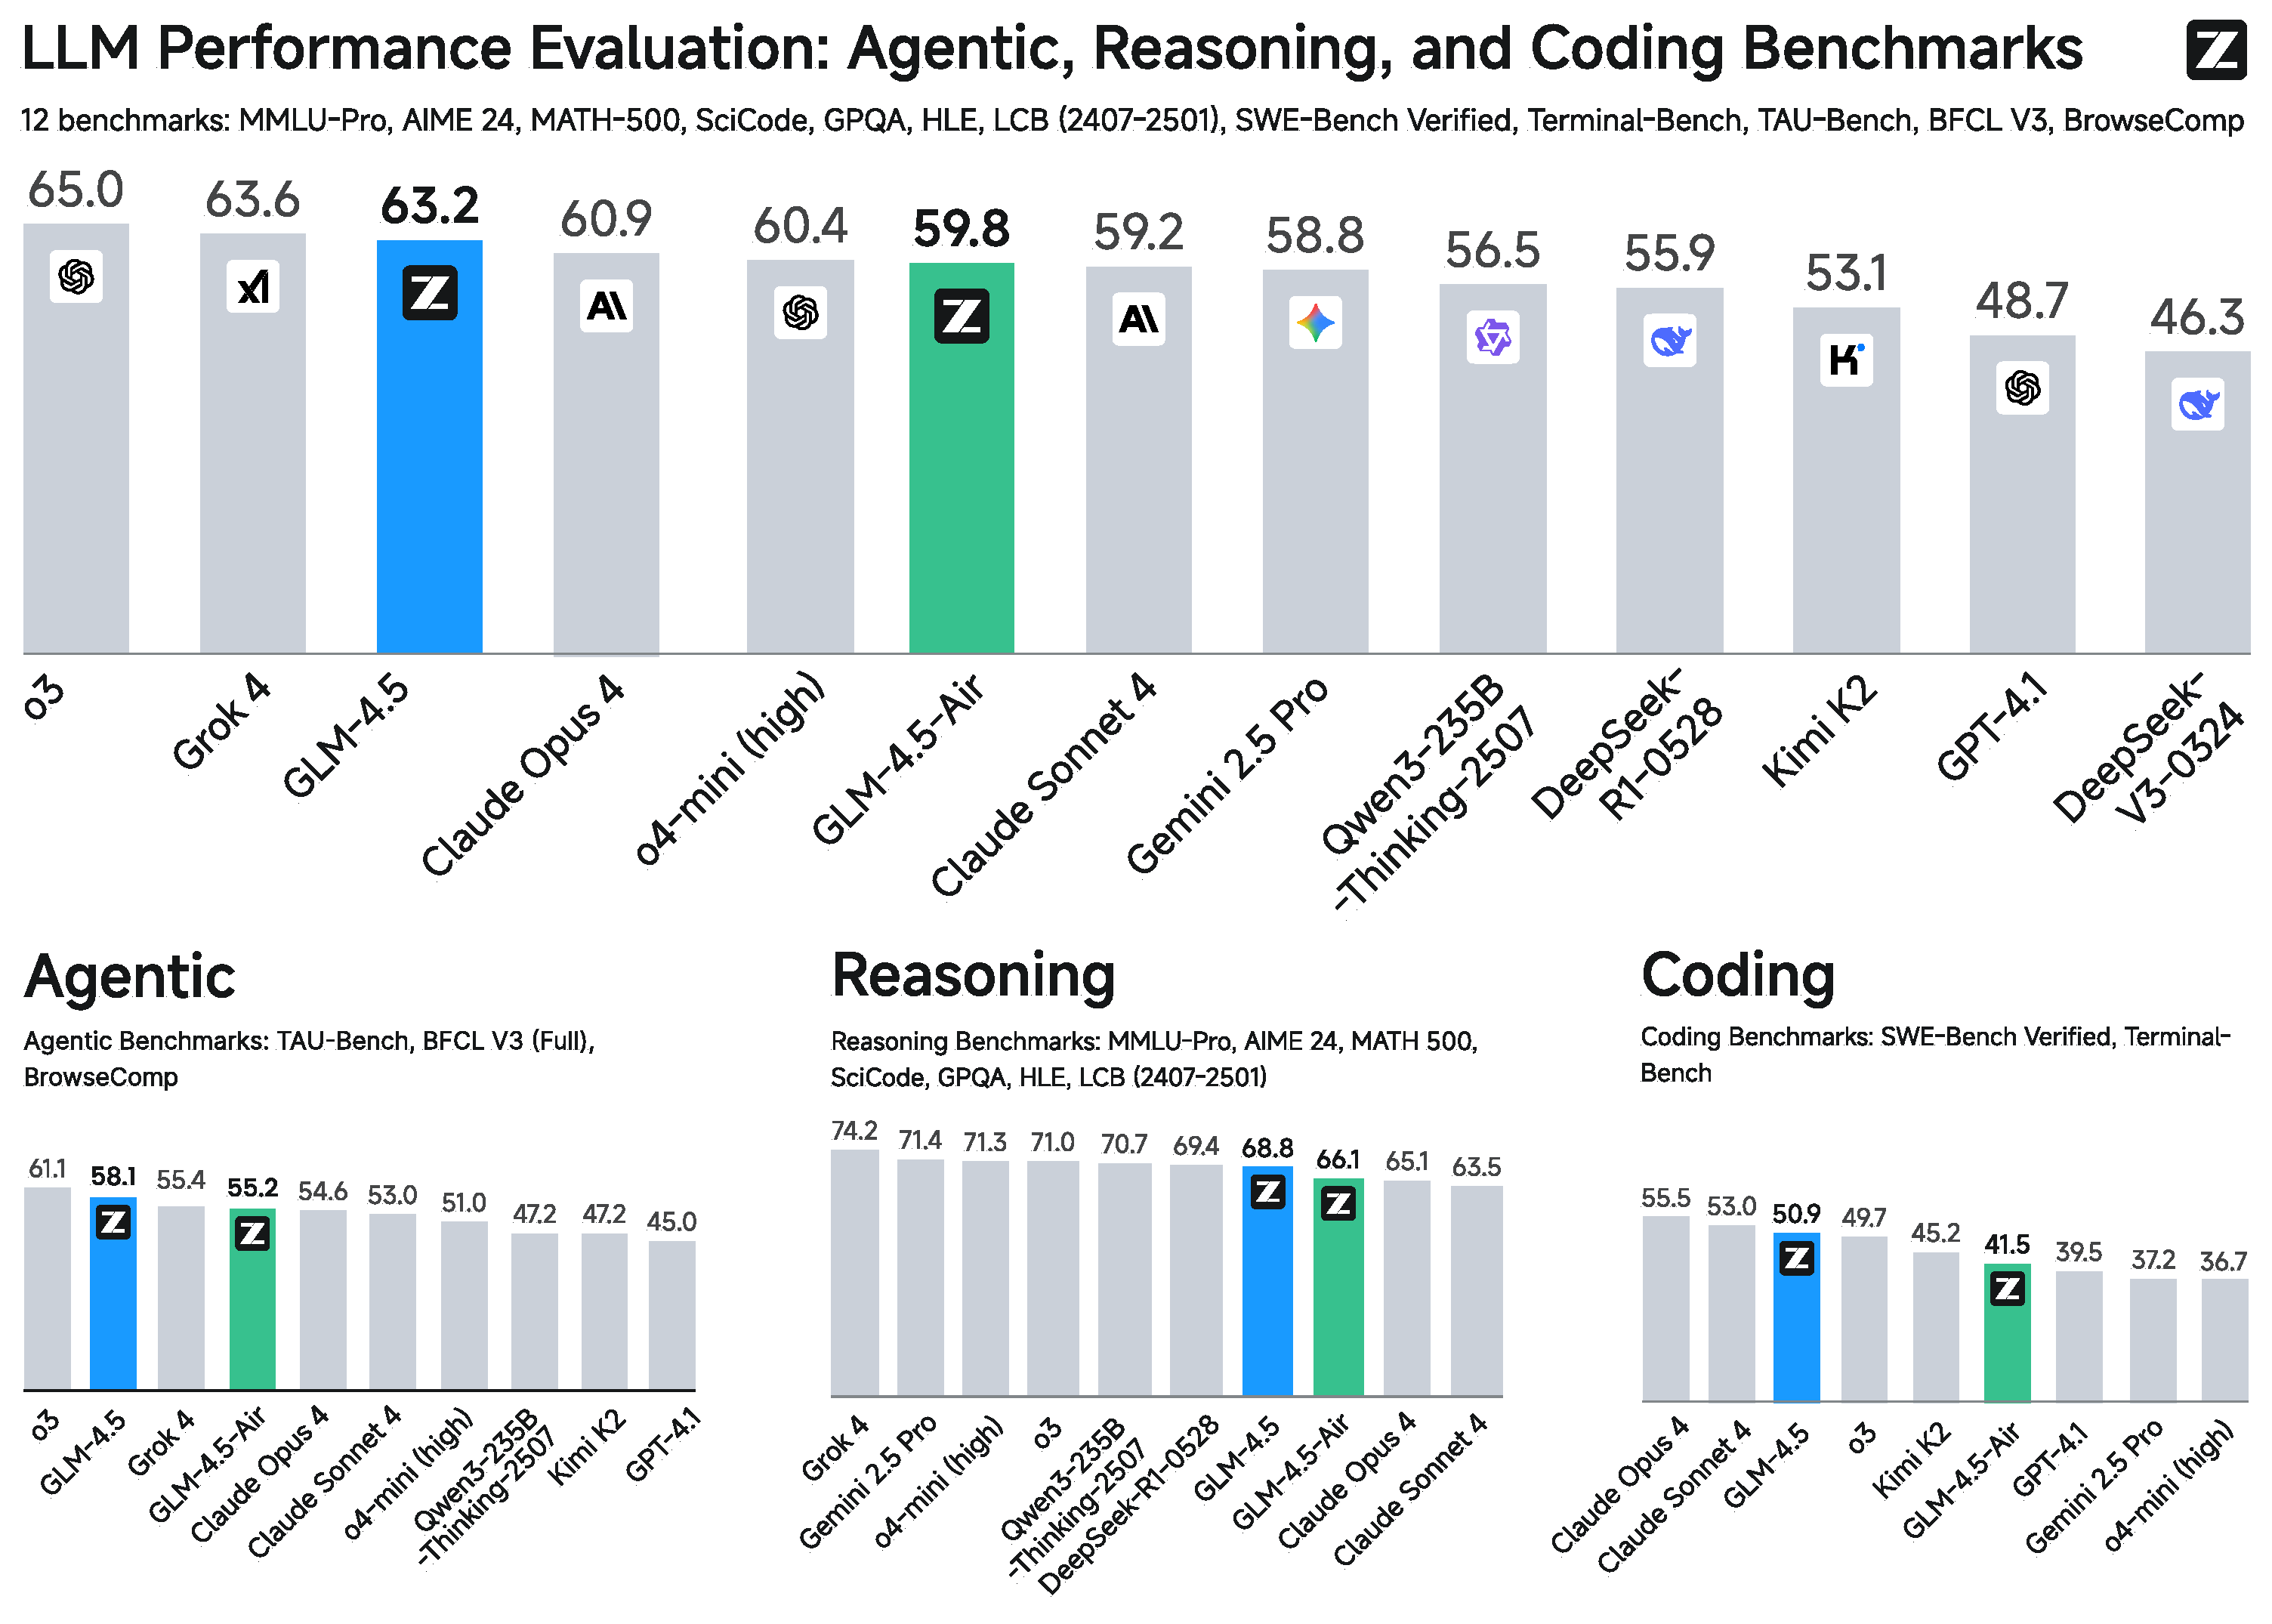
\includegraphics[width=0.925\linewidth]{figures/arc_benchmark.pdf}
    \caption{
    Average performance on agentic, reasoning, and coding (ARC) benchmarks. Overall, GLM-4.5 achieves a rank of 3rd, with GLM-4.5-Air following at rank 6th.
    The models listed are evaluated as of July 28, 2025.
    }
    \label{fig:arc_benchmark}
\end{figure}

\section{Introduction}

% Large language models (LLMs)~\cite{brown2020language,touvron2023llama,zengglm,team2023gemini,liu2024deepseek} learn general knowledge from large-scale web corpora.
% %and boost popular applications like ChatGPT. 
% The ultimate goal of LLMs, or even so-called AGI, is to achieve human-level cognitive capabilities across a wide range of domains, rather than being designed for specific tasks. 
% In other words, a good LLM should be able to deal with general problem-solving, generalization, commonsense reasoning, and self-improvement at the same time.
% With the applications of LLMs deepen in our daily life, new challenges arise that drives the development of models. First, language models often fail to solve complex problems that require long reasoning processes, such as math Olympiad questions and programming problems on Leetcode and Codeforces. OpenAI o1~\cite{jaech2024openai} uses reinforcement learning to optimize the textual reasoning processes of language models, achieving 74\% accuracy on AIME 2024 and 89\% accuracy on Codeforces. Second, coding in real-world scenarios poses challenges to language models. Although language models can implement a single function given the docstring~\cite{chen2021evaluating}, it is much more challenging to complete software engineering tasks such as fixing a bug or implementing a new feature in an existing project with multiple files and directories. Anthropic's Claude Opus 4 achieves 70.4\% accuracy on SWE-bench Verified~\cite{jimenez2023swe}, a benchmark that measures a language model's ability to resolve GitHub issues. Third, to gather the latest information and take real-world actions, language models need to call external tools. Language models equipped with various tools to perform specific tasks are often denoted as agents. Agentic tasks require language models to choose appropriate tools, provide correct parameters, and reflect previous actions based on execution results.

% Looking backward, OpenAI's GPT-3 has learned commonsense knowledge, and OpenAI o1 uses reinforcement learning to think before responding, significantly improving reasoning skills in coding, data analysis, and complex math. However, the resultant models are still not really general: some of them are good at coding, some good at math, and some good at reasoning, but none of them can achieve the best performance across all the different tasks.

Large language models (LLMs) are rapidly evolving from general knowledge repositories~\cite{brown2020language,touvron2023llama,zengglm,team2023gemini,liu2024deepseek} into general problem-solvers. The ultimate ambition, often associated with Artificial General Intelligence (AGI), is to create models with human-level cognitive capabilities across diverse domains. This requires a unified mastery of complex problem-solving, generalization, and self-improvement, moving beyond task-specific excellence.

As LLMs become more integrated into real-world scenarios, the key to enhancing actual productivity and solving complex professional tasks lies in developing specific core capabilities.
We identify three critical, interconnected capabilities as the measure of a truly generalist model: \textbf{Agentic} abilities for interacting with external tools and the real world; complex \textbf{Reasoning} for solving multi-step problems in domains like mathematics and science; and advanced \textbf{Coding} skills for tackling real-world software engineering tasks. While state-of-the-art proprietary models like OpenAI's o1/o3~\cite{jaech2024openai} and Anthropic's Claude Sonnet 4 have demonstrated groundbreaking performance in specific ARC domains (e.g., mathematical reasoning or code fixing~\cite{jimenez2023swe}), a single, powerful open-source model that excels across all three areas has remained elusive.

This paper introduces two new models: GLM-4.5 and GLM-4.5-Air, toward the goal of unifying all the different capabilities.
The new models outperform existing open-source LLM models~\cite{guo2025deepseek,team2025kimi,yang2025qwen3} across the board, with significant gains in agentic, reasoning, and coding tasks. GLM-4.5 and GLM-4.5-Air both feature hybrid reasoning modes: thinking mode for complex reasoning and agentic tasks, and non-thinking mode for instant responses. GLM-4.5 is our first MoE model, with 355B total parameters and 32B activated parameters. GLM-4.5 demonstrates strong performance on the following ARC benchmarks:

\begin{itemize}[leftmargin=*,itemsep=0pt,parsep=0.4em,topsep=0.0em,partopsep=0.0em]
     \item \textbf{Agentic:} GLM-4.5 scores 70.1\% on TAU-Bench and 77.8\% on BFCL v3~\cite{patil2025bfcl}, on par with Claude Sonnet 4. For web browsing agents, GLM-4.5 scores 26.4\% on BrowseComp~\cite{wei2025browsecomp}, clearly outperforming Claude Opus 4 (18.8\%) and close to o4-mini-high (28.3\%).
     
    \item \textbf{Reasoning:} GLM-4.5 demonstrates outstanding performance on a suite of challenging reasoning benchmarks, achieving 91.0\% on AIME 24, 79.1\% on GPQA~\cite{rein2024gpqa}, 72.9\% on LiveCodeBench (2407-2501)~\cite{jainlivecodebench}, and 14.4\% on HLE (Humanity's Last Exam)~\cite{phan2025humanity}.
    
    \item \textbf{Coding:} GLM-4.5 scores 64.2\% on SWE-bench Verified~\cite{jimenez2023swe} and 37.5\% on Terminal-Bench~\cite{tbench_2025}, outperforming GPT-4.1 and Gemini-2.5-pro, close to Claude Sonnet 4.
\end{itemize}

GLM-4.5-Air is a smaller MoE model with 106B parameters. It represents a significant leap among models at the 100B scale, matching or exceeding Qwen3-235B-A22B~\cite{yang2025qwen3} and MiniMax-M1~\cite{chen2025minimax}.

In \Cref{fig:arc_benchmark}, we show the average performance on 12 benchmarks across agentic, reasoning, and coding (ARC) tasks. Overall, GLM-4.5 is ranked in the \textbf{3rd} place and GLM-4.5-Air is ranked in the \textbf{6th}. On agentic tasks, GLM-4.5 is ranked in the 2nd place, following OpenAI o3. On coding tasks, GLM-4.5 is ranked in the third place, close to Claude Sonnet 4. Note that GLM-4.5 is highly parameter-efficient, with only half the parameters of DeepSeek-R1~\cite{guo2025deepseek} and one-third those of Kimi K2~\cite{team2025kimi}. In \Cref{fig:swe-parameter}, we report the scores on SWE-bench Verified vs model parameters of different open-source models, where GLM-4.5 and GLM-4.5-Air lie on the Pareto Frontier.
%, achieving the best performance on the same scale. 
More evaluation results are detailed in~\Cref{sec:evaluation}.

Both GLM-4.5 and GLM-4.5-Air are available on \url{Z.ai}, \url{BigModel.cn}, and also as open-source models on \url{https://huggingface.co/zai-org/GLM-4.5}. We also open-sourced an evaluation toolkit at \url{https://github.com/zai-org/glm-simple-evals} to ensure the reproducibility of our benchmark results.

\begin{figure}
    \centering
    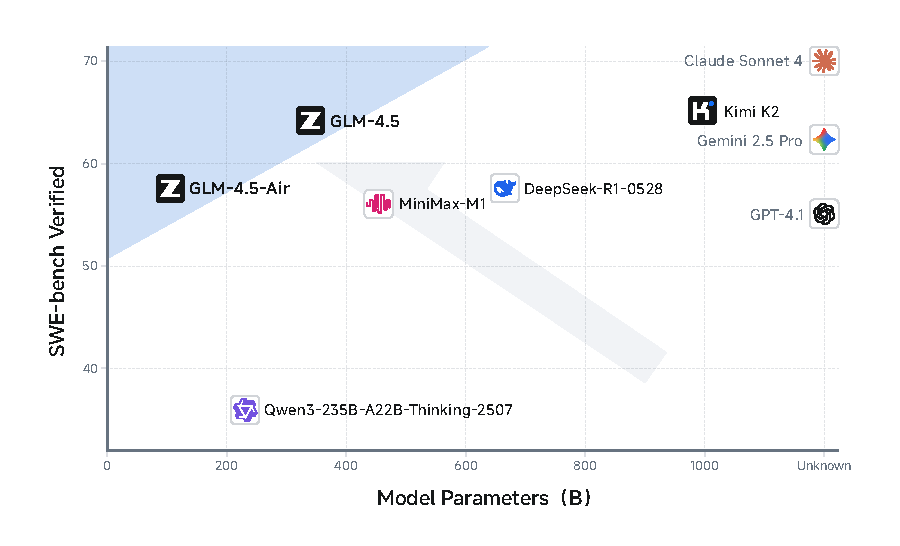
\includegraphics[width=0.9\linewidth, trim=0 15 0 15, clip]{figures/swe_parameter.pdf}
    \caption{SWE-bench verified scores vs model parameters. Proprietary models are listed as unknown at the right side.}
    \label{fig:swe-parameter}
\end{figure}